\documentclass[a4paper]{article}%[fleqn] kan vara snyggt
\usepackage{custom}

\begin{document}
\title{Nollställena till Riemanns Zeta-funktion och dess Beteende på den Kritiska Linjen}
\author{Linus Bergkvist}
\date{}
\maketitle

\pagebreak
\section*{Introduktion}
Riemannhypotesen beskrevs för första gången 1859 av Bernhard Riemann och lyder:
Alla icke-triviala nollställen till Riemanns Zeta-funktion har Realdelen $\frac 1 2$.
För \smash{$\mRe{s} > 1$} definieras Riemanns Zeta-funktion som $\sum\limits_{n = 1}^\infty \frac 1 {n^s}$. 
För att kunna studera dess nollställen i det komplexa talplanet måste man alltså först hitta
ett sätt att beskriva Zeta-funktionen på som gäller för alla $s$ i $C$. 
Arbetet är i huvudsak uppdelat i 2 delar och ett Appendix. I den första delen begränsas 
Zeta-funktionens icke-triviala nollställen till en ``remsa'' i det komplexa talplanet 
(de triviala nollställena $(-2, -4, -6, -8\ldots)$ får också sin förklaring). 
I den andra delen studeras nollställena längs den ``kritiska linjen'' $(\frac 1 2 + it,\quad t \in \mathbb{R})$.
Det finns även ett appendix i vilket vissa, inte helt uppenbara satser som används i arbetet, härleds.

\newcommand{\mres}{
	\mRe{s}
}

\newcommand{\zfn}{
	zeta-funktionen
}

\section*{Del 1}
I denna del kommer det först att bevisas att zeta-funktionen inte har några nollställen för $\mres > 1$.
Därefter påvisas en funktion som har samma nollställen som zeta-funktionen, och som därefter bevisas
vara invariant från $s \to (1 - s)$. Av denna invarians följer det att zeta-funktionen omöjligt kan 
ha några icke-triviala nollställen för $\mres < 0$. Därefter visas en funktion som på linjen $1 + it$, har
samma nollställen som \zfn. Därefter visas det att denna funktion inte har något nollställe för något värde
på $t$, vilket har som följd att \zfn inte har några nollställen på linjen $\mres = 1$ Därefter följer det 
av den sedan tidigare påvisade invariansen att \zfn inte heller har några nollställen på linjen $\mres = 0$.
Sammanfattningsvis har alltså zeta-funktionens nollställen begränsats till remsan $0 < \mres < 1$.\\
\\
\paragraph{Sats 1:}
Det finns inga nollställen till Riemanns zeta-funktion med Realdelen $> 1$.\\
\\
{\bf Bevis:} \\
För $s$ med $\mRe{s} > 1$ definieras Riemanns zeta-funktion som 
$\zeta(s) = \sum\limits_{n = 1}^\infty \frac {1} {n^s}$ 
\begin{equation}
	\begin{aligned}
		&\zeta(s) = \frac 1 {1^s} + \frac 1 {2^s} + \frac 1 {3^s} + \frac 1 {4^s} \ldots \notag\\
		&\zeta(s) \cdot \frac 1 {2^s} = \frac 1 {2^s} + \frac 1 {4^s} + \frac 1 {6^s} + \frac 1 {8^s} \ldots \\
		&\zeta(s) - \frac {\zeta(s)} {2^s} = \frac 1 {1^s} + \frac 1 {3^s} + \frac 1 {5^s} \ldots &
		\hspace{\width} &\text{Vi har nu tagit bort alla multiplar av } \frac 1 {2^s} \\
		&\zeta(s) (1 - \frac 1 {2^s}) \cdot \frac 1 {3^s} = \frac 1 {3^s} + \frac 1 {9^s} + \frac 1 {15^s} \ldots\\
		&\zeta(s)(1 - \frac 1 {2^s})(1 - \frac 1 {3^s}) = \frac 1 {1^s} + \frac 1 {5^s} + \frac 1 {7^s} \ldots &
		\hspace{\width} &\text{Vi har nu tagit bort alla} \\
		& & \hspace{\width} &\text{återstående multiplar av } \frac 1 {3^s} \\
	\end{aligned}
	\phantom{\hspace{4cm}}
\end{equation}
Om man gör så med alla primtal får man: 
\begin{equation}
	\begin{aligned}
		\notag
		&\zeta(s) \cdot (1 - \frac 1 {2^s})(1 - \frac 1 {3^s})(1 - \frac 1 {5^s}) \ldots = \frac 1 {1^s} = 1 \Leftrightarrow \\  
		&\zeta(s)  = \frac 1 {(1 - \frac 1 {2^s})(1 - \frac 1 {3^s})\ldots} = \prod_p \frac 1 {1 - p^{-s}}.\hspace{\width} \mRe{s} > 1 \\
		&\frac {\zeta(s)} {\displaystyle\prod_p \frac 1 {(1 - p^{-s})}} = 1 = \zeta(s) \cdot \prod_p (1 - p^{-s}) \\
	\end{aligned}
\end{equation}
Då $s = a+ bi$ ger att $1-p^{-s} = 1 - e^{-\ln(p) \cdot a} \cdot e^{-ln(p) \cdot bi}$, vilket för $a > 1$ har
absolutbelopp $\leq 1$ följer det att produkten inte har några singulariteter. 
Vilket visar att $\zeta(s) \ne 0 \text{ För } \mRe{s} > 1$\\

\paragraph{Definition:}
Den kompletta zeta-funktionen.\\
\[
	\xi (s) = \frac 1 2 \cdot s(s - 1) \cdot \pi^{-s/2} \cdot \Gamma(\frac s 2) \cdot \zeta(s) 
\]
där
\[
	\Gamma(s) = \int_0^\infty t^{s - 1} \cdot e^{-t}\; dt
\]

%\pagebreak
\paragraph{Sats 2:} Den kompletta zeta-funktionens nollställen är nollställen för Riemanns zeta-funktion.\\
\\
{\bf Bevis:}\\
Det här är ett väldigt kort bevis. Eftersom varken ${\frac 1 2 \cdot s, (s - 1), \pi^{-s/2}}$ eller $\Gamma(\frac s 2)$
har några nollställen utöver punkterna $s = 0$ och $s = 1$ så måste $\xi(s)$ ha samma nollställen som $\zeta(s)$.

\paragraph{Sats 3:} $\xi(s) = \xi(1 - s)$. \\
\\
{\bf Bevis:}\\
\newcommand{\myG} {
	\Gamma(\frac s 2) = \int_0^\infty
}
\[
	\myG t^{s/2 - 1} \cdot e^{-t}\; dt
\]
Vi gör substitutionen $t = \pi \cdot n^2 \cdot x$.
\[
	\myG \pi^{(s/2 - 1)} \cdot n^{2^{(s / 2 - 1)}} \cdot x^{(s/2 - 1)} \cdot e^{-\pi \cdot n^2 \cdot x}\; dx
\]
\[
	\pi^{-s/2} \cdot \Gamma(\frac s 2) \cdot n^{-s} = \int_0^\infty x^{s/2 - 1} \cdot e^{-\pi n^2 x}\; dx
\]
Vi vet att $\zeta(s) = \sum\limits_{n \ge 1} n^{-s}$\\
Vi summerar båda leden över n med $n>0$ och erhåller då:\\
$$\sum_{n \ge 1} \pi^{-s/2} \cdot \Gamma(\frac s 2) \cdot n^{-s} = \pi^{-s/2} \cdot \Gamma(\frac s 2) \cdot \zeta(s) = 
\int_0^\infty x^{s/2 - 1} \cdot \sum_{n \ge 1} e^{-\pi n^2 x}\; dx$$
framöver betecknar vi $\sum\limits_{n \ge 1} e^{-\pi x n^2} \text{ som } \omega(x)$.
Nu delar vi upp integralen vid $1$ och erhåller:%linus skrev får istället för erhåller
\[
	\int_0^1 x^{s/2 - 1} \cdot \omega(x)\; dx + \int_1^\infty x^{s/2 - 1} \cdot \omega(x)\; dx
\]
För att få samma integrationgränser i de båda integralerna gör vi substitutionen $x = x^{-1}$ i den första integralen och erhåller då:
\[
	\int_1^\infty x^{-s/2 - 1} \cdot \omega(x^{-1})\; dx + \int_1^\infty x^{-s/2 - 1} \cdot \omega(x)\; dx
\]
Vi definierar nu funktionen $\theta(x)$ som:
\[
	\theta(x) = \sum_{n \in \mathbb{Z}} e^{-xn^2\pi}
\]
Eftersom $n^2=(-n)^2$ och $e^{-x0^2\pi} = 1$ får vi att 
\[
	\theta(x) = 2\omega(x) + 1
\]
Vi använder nu Fouriertransformen på $e^{-\pi n^2 x}$ och erhåller
\[
	\mathcal{F}(e^{-\pi n^2 x})(u) = x^{-1/2} \cdot e^{-\pi u^2/x}
\]
Vi använder därefter summationsformeln från Sats 1 i appendix och erhåller då:
\[
	\theta(x) = x^{-1/2}\theta(x^{-1})
\]
\[
	2\omega(x) + 1 = \frac {
		1
	} {
	\sqrt{x}
	} 
	(2\omega(x^{-1}) + 1) \Leftrightarrow 
		\omega(x^{-1}) = \omega(x) \cdot \sqrt{x} + 
			\frac {
				\sqrt{x}
			}
			2 - \frac 1 2
\]
Om vi nu använder vårt uttryck för $\omega(x^{-1})$ i den tidigare integralen erhåller vi:
\[
	\int_1^\infty x^{-s/2 - 1} \cdot 
	\omega(x^{-1})\; dx = 
	- \frac 1 s + \frac 1 {s - 1} + 
	\int_1^\infty x^{(s + 1)/2} \cdot
	\omega(x)\; dx
\]
Och hela ekvationen blir då:
\[
	\xi(s) = \pi^{-s/2} \cdot 
	\Gamma(\frac s 2) \cdot 
	\zeta(s) = - \frac 1 {s(1 - s)} + 
	\int_1^\infty(x^{s/2 - 1} + 
	x^{-(s + 1)/2}) \cdot \omega(x)\; dx
\]
Om vi byter ut $s$ mot $(1 - s)$ i det högra uttrycket erhåller vi samma uttryck igen. Därför gäller det att $\xi(s) = \xi(1 - s)$ \\
\hfill \qed\\
(Division med $\Gamma(\frac s 2 )$ i den sista likheten, innebär att zeta-funktionen har nollställen varje gång då $\Gamma(\frac s 2 )$ har en singularitet. På så sätt erhålls de ``triviala nollställena'')
\pagebreak
\paragraph{Sats 4:} De triviala nollställena till Riemanns zeta-funktion är de enda nollställena utanför intervallet $0 < \mRe{s} < 1$.\\
\\
{\bf Bevis:}\\ %Skrivas i obestämd form ex. I Sats 1 bevisades att \ldots?
I Sats 1 bevisades det att $\zeta(s)$ inte har några nollställen för $\zeta(s)$ och i Sats 3 bevisades det att $\xi(s) = \xi(1 - s)$.
Om vi antar att det finns en punkt p med $\mRe{p} < 0$ sådan att $\zeta(p) = 0$ innebär det av Sats 2 att $\xi(p) = 0 \Leftrightarrow
\xi(1 - p) = 0 \Leftrightarrow \zeta(1 - p) = 0$ men om $\mRe{p} < 0$ är $\mRe{1 - p} > 1$. Då innebär det att det finns en punkt
$q = 1 - p$ med $\mRe{q} > 1$ sådan att $\zeta(q) = 0$. Men detta strider mot Sats 1. Det kan alltså inte finnas en punkt $p$ med
$\mRe{p} < 0$ sådan att $\zeta(p) = 0$. \\
\hfill \qed %Ska skrivas om så att ekvationerna inte linebreakas
%I slutet på andra meningen i stas 5 så ska det stå "med \operatorname{Re} > 1"
%efter zetat. vilket zeta?

\paragraph{Sats 5:} $\zeta(s + it) = 0$ for $s = 1$ omm $\zeta(s)^3 \cdot \zeta(s + it)^4 \cdot \zeta(s + 2it) = 0$ \\
för $s = 1$. \\
\\
{\bf Bevis:}\\
$\zeta(s)$ har en singularitet för $s = 1$. Men eftersom faktorn $\zeta(s + it)^4$ är av högre grad kan singulariteterna
för $\zeta(s)$ inte ta ut ett eventuellt nollställe. Termen $\zeta(s + 2it)$ kan bli $0$, men då den aldrig kan bli en 
singularitet kan den inte ta ut ett eventuellt nollställe.\\
\hfill\qed\\
\paragraph{Hjälpsats 6:} $\ln(1 - i) = - \sum\limits_{n = 1}^\infty \frac {x^n} n$ \\
\\
{\bf Bevis:}\\
\[
	f(x) = \ln(1 - x) \Rightarrow f(0) = \ln(1) = 0
\]
Definitionen av Maclaurinpolynom är:
\newcommand{\mymac}[1] {
	f(x) = \sum_{n = #1}^\infty \frac {
		f^{(n)}(0) \cdot x^n
	} {
		n!
	}
}
\[
	\mymac{0}
\]
men då $\ln(1) = 0$ är:
\[
	\ln(1 - x) = \mymac{1}
\]
Derivering ger att
\begin{align*}
	&f^{(n)}(0) = -(n - 1)! \\
	&\Downarrow \\ 
	&\ln(1 - x) = \sum_{n = 1}^\infty \frac {-(n - 1)! \cdot x^n} {n!} =
			- \sum_{n = 1}^\infty \frac {x^n} n
\end{align*}
\hfill \qed

\newcommand*{\ps}{1 - p^{-s}}
\paragraph{Sats 7:} $\zeta(s)$ har inga nollställen för $\mRe{s} = 1$. \\
\\
{\bf Bevis:}\\
Vi använder oss av ett uttryck från Sats 1:
\[
	\zeta(s) = \prod_p \frac 1 {1 - p^{-s}}
\]
\[
	\ln (\frac 1 {
		1 - p^{-s}
	})
	= \ln(1) - \ln(1 - p^{-s}) = -\ln(1 - p^{-s})
\]
\[
	\ln \left |
		\zeta(s)
	\right | = \ln \left |
		\prod_p \frac 1 {1 - p^{-s}}
	\right |
	= \sum_p \ln \left | 
		\frac 1 {1 - p^{-s}} 
	\right |
	= - \sum_p \ln \left |
		1 - p^{-s}
		\right | = - \mRe{\sum_p \ln(\ps)
\] 
Hjälpsats 6 ger nu:
\[
	-\mRe{\sum_p \ln(\ps)} 
	= (\sum_p \sum_{n = 1}^\infty(
		\frac {p^{-ns}} n
	)}
\]
Vi definierar nu $h(x) = \zeta(x)^3 \cdot \zeta(x + it)^4 \cdot \zeta(x + 2it)$, logaritmlagarna ger nu:
\begin{align*}
	\ln(h(x)) &= 3 \ln \left | \zeta(x) \right | + 4 \ln \left | \zeta(x + it) \right | + \ln \left | \zeta(x + 2it) \right |\\  
			 &= \sum_p \sum_{n = 1}^\infty \frac 1 n \cdot p^{nx} \cdot \mRe{3 + 4p^{-int} + p^{-int \cdot 2}} 
\end{align*}
eftersom:
\[
	\frac 1 n \cdot p^{-nx} \ge 0
\]
följer det att det vi måste undersöka är om \\
\[
	\operatorname{Re}(3 + 4p^{-int} + p^{-2int}) \ge 0
\]
\\
\[
	p^{-int} = e^{\ln(p) \cdot -int}
\]
\[
	\theta = -\ln(p) \cdot n \cdot t \Rightarrow
	e^{i\theta} \Rightarrow
	\operatorname{Re}(3 + 4 \cdot e^{i\theta} + e^{i2\theta})
\]
Eulers formel ger nu:
\[
	\operatorname{Re}(3 + 4e^{i\theta} + e^{2i\theta})
		= 3 + 4\cos(\theta) + \cos(2\theta)
\]
likheten $\cos(2\theta) = 2\cos^2(\theta) - 1$ ger:
\[
	3 + 4 \cos(\theta) + 2 \cos^2(\theta) - 1 
		= 2(1 + 2\cos(\theta) + \cos^2(\theta)) 
		= 2(1 + \cos(\theta))^2 \ge 0
\]
alla termer i vår summa är alltså större eller lika med 0. Då exempelvis\\
$\theta = -\ln(2) \cdot 2$ ger en term $ > 0$ innebär detta att summan är strikt större än 0.\\
%w00t? nej om $f(x) = \sum_0^\infty g(x), g(x) \ge 0 är f(x) också \ge 0$
Det finns alltså inga nollställen för $\zeta(s)$ med $\mRe{s} = 1$.\\
\hfill \qed

\paragraph{Sats 8:} Det finns inga nollställen för $\zeta(s)$ med $\mRe{s} = 0.$\\
\\
{\bf Bevis:}\\
Sats 2 och 3 visar att om $\zeta(s)$ är ett nollställe är $\zeta(1 - s)$ också det.
Om det finns något $\zeta(0 + it) = 0$ följer även att $\zeta(1 - (0 + it)) = \zeta(1 - it) = 0$. Men detta 
motbevisades i Sats 7.\\
Notera att Sats 2 inte fungerar i punkterna $s = 1$ och $s = 0$. Med då $\zeta(0) = -\frac 1 2$ och 
$\zeta(1) = \infty$ håller Satsen.
\hfill \qed
\pagebreak
\newcommand{\zit}{
	$\zeta(\frac 1 2 + it)$
}
\section*{Del 2}
I denna del så utgår man från ett uttryck av 2 variabler som bland annat innehåller \zit, som
därefter, genom flera hjälpsatser, skrivs om till ett annat uttryck. Detta uttryck förändras i sin tur
genom derivering med avseende på en av variablerna. Genom ett motsägelsebevis visas det därefter
slutligen att denna derivata omöjligt kan sluta växla tecken för $t > T$ för något stort $T$. Då den enda
funktionen i uttrycket som potentiellt sett kan växla tecken oändligt många gånger är \zit 
följer det därav att \zfn har oändligt många nollställen på den kritiska linjen.\\
\\
\paragraph{Sats 9:} Om $\zeta(s) = 0$ för något tal $s = \frac 1 2 + it$ med $t \in \mathbb{R}$ är $\zeta(\overline{s}) = 0$ \\
\\
{\bf Bevis:}\\
Det har tidigare visats att om $\zeta(s) = 0$ är $\zeta(1 - s) = 0$. $\zeta(\frac 1 2 + it) = 0 \Leftrightarrow 
\zeta(1 - (\frac 1 2 + it)) = \zeta(\frac 1 2 - it) = 0$
\hfill \qed

\paragraph{Definition: Mellintransform} $\{\mathcal{M}f\}(s) = \varphi(s) = \int_0^\infty x^{s - 1} \cdot f(x) \; dx $ \\
\\
Mellintransformen har inversionsformen
\[
	f(x) = \frac {1} {2 \pi i} \cdot \smartint{C}{i \infty}
		x^{-s} \cdot \varphi(s) \; ds
 \]

\paragraph{Hjälpsats 10:} 
\[
	\{\mathcal{M} \omega \} (x) = \zeta(2s) \cdot \Gamma(s) \cdot \pi^{-s}
\]
med 
\[
	\omega(y) = \sum\limits_{n \leq 1} e^{-n^2\pi y}
\]
\\
{\bf Bevis:} \\ 
Denna likhet härleddes i Sats 3, men då utan beteckningen Mellintransform.\\
\\
\paragraph{Hjälpsats 11:} 
\[
	\omega(y) = \frac {1} {2\pi i} \smartint{C}{i \infty} \zeta(zs) \cdot \Gamma(s) \cdot \pi^{-s} \cdot
		y^{-s} \; ds \text{ för } c > \frac 1 2
\] 
\\
{\bf Bevis:}\\
Detta följer av att applicera Mellintransformens inversionsformel på Hjälpsats 10.\\

\paragraph{Definition:} $\Xi(t) = \zeta(\frac 1 2 + it)$ \\
\\
\newcommand{\helper}[1] {
	\int_#1^\infty (t^2 + \frac 1 4)^{-1}
}
\newcommand{\twelve}[1][0] {
	\helper{#1} \cdot \cos(xt) \; dt
}
\paragraph{Sats 12:} 
\[
	\twelve = \frac 1 2 \pi(e^{\frac 1 2 x} -
		2e^{-\frac 1 2 x} \omega(e^{- 2 x}))
\]
{\bf Bevis:}\\
\[
	\text{Sätt } Q(x) = \twelve
\]
Då $(t^2 + \frac 1 4) \cdot \Xi(t) \cdot \cos(xt)$ är symmetrisk kring $t = 0$ (se Sats 9 för $\Xi(t)$'s symmetri)
så gäller:
\newcommand{\mQ} {
	\frac 1 2 \twelve{\infty}
}
\[
	Q(x) = \mQ \quad (1)
\]
Då $\sin(xt)$ är ``inverst symmetrisk'' kring $t = 0$ följer det att 
\[
	\mQ = 0 \quad (2)
\]
Addition av $(1)$ och $(2)$ tillsammans med Eulers formel ger nu: 
\[
	Q(x) = \frac 1 2 \cdot \helper{-\infty} \Xi(t)\cdot e^{ixt} \; dt
\]
låt $s = \frac 1 2 + it$. Då följer:
\[
	Q(x) = \frac {
		e^{- \tfrac 1 2 x t}
	} {
		2i
	} \cdot \smartint{\tfrac 1 2}{\infty}
		\frac {1} {s(1-s)} \Xi(s) \cdot e^{xs} \; ds
\]
Definitionen av $\zeta(s)$ ger nu:
\[
	Q(x) = - \frac {
		e^{- \frac 1 2 xt}
	} {
		4i
	} \cdot \smartint{\tfrac 1 2}{\infty} \zeta(s) \cdot \Gamma
		\pi^{- \frac s 2} \cdot e^{xs} \; ds
\]
$z(s) \cdot \Gamma(\frac s 2) \pi^{- \frac s 0} \cdot e^{xs}$ har singulariteter i $s = 0$ och $s = 1$.
Därmed följer det att om vi flyttar linjeintegralen till höger om linjen $c=1$ så korrigeras förändringen med att 
subtrahera residualen i $s = 1$ så för $c > 1$ gäller:
\[
	Q(x) = - \frac {e^{- \frac 1 2 xt}} {4i} \cdot \int_{\tfrac 1 2 - \infty}^{\tfrac 1 2 + \infty} \zeta(s) \cdot \Gamma
		\pi^{- \frac s 2} \cdot e^{xs} \; ds + \frac {e^{- \frac 1 2 xt}} {4i} \cdot2 \pi i \cdot \operatorname{Res}(\zeta(s) \cdot
		\Gamma(\frac s 2) \cdot \pi^{-\frac s 2} \cdot e^{xs}, 1)
\]
Då $\operatorname{Res}(\zeta(s), 1) = 1$ (se Appendix Sats 14) följer det att:
\[
	\frac {e^{- \frac 1 2 x}} {4i} \cdot 2 \pi i \cdot 1 \cdot \Gamma(\frac 1 2) \cdot \pi^{- \frac 1 2} \cdot e^x =
		\frac {e^{\frac 1 2 x}} {2} \cdot \pi \cdot 1 \cdot \sqrt{x} \cdot \frac {1} {\sqrt{x}} = \frac {e^{\frac 1 2 x} \pi} {2}
\]
Därmed följer:
\[
	Q(x) = - \frac {e^{-\frac 1 2 x}} {4 i} \cdot \int_{C - \infty}^{C + \infty} \zeta(s) \cdot \Gamma(\frac s 2)
		\cdot \pi^{- \frac 1 2} \cdot e^{xs} \; ds + \frac \pi 2 \cdot e^{\frac 1 2 x}
\]
genom att sätta $y = e^{-2x}$ erhålls det från Hjälpsats 11 att:
\[
	Q(x) = - \pi e^{- \frac 1 2 x} \cdot \omega(e^{- 2 x}) + \frac \pi 2 e^{\frac 1 2 x} = \frac 1 2 \pi
		(e^{\frac 1 2 x} - 2 e^{- \frac 1 2 x} \cdot \omega(e^{-2x}))
\]
\hfill \qed

\paragraph{Hjälpsats 13:} För alla heltal $n$ gäller:
\[%vad är det här?
	\lim_{a \to \frac n 4 \pi^+} \frac {
		d^{2n} [
			e^{\frac 1 2 ia} (\frac 1 2 + \omega(e^{2ia}))
		]}
		{
			da^{2n}
		} = 0
\]
\\
{\bf Bevis:}\\
Observera att:
\newcommand{\mysum} {
	\sum_{n = 1}^\infty e^{-n^2 v \pi} \cdot
}
\begin{align*}
	\omega(i + v) &= \sum_{n = 1}^\infty e^{-n^2 \pi(i + v)} \\
		&= \mysum e^{-\pi i n^2} \\
		&= \mysum (- 1)^{n^2} \\
		&= \mysum (- 1)^n
\end{align*}
Det sista steget gäller då udda $n$ ger udda $n^2$ och jämna $n$ ger jämna $n^2$.
\[
	2 \omega(4v) - \omega(v) = \sum_{n = 1}^\infty 2 e^{-n^2 \pi 4 v} - e^{-n^2 \pi v} = \sum_{n = 1}^\infty 2
		e^{-(2n)^2\pi v} - e^{-n^2 \pi v} 
\]
\[
	= \sum_{n = 1}^\infty (-1)^n \cdot e^{-n^2 vt} = \omega(i + v) = 2 \omega(4 v) -
			\omega(v) \qquad (1)
\]
\[
	\omega(x) x^{- \frac 1 2} \cdot \omega(\frac 1 x) + \frac 1 2  x^{- \frac 1 2} - \frac 1 2 \text{ (Se Sats 3 för härledning)}
\]
Vilket ger att $(1)$ blir:
\[
	\omega(i + v) = \frac {1} {\sqrt v} \cdot \omega(\frac {1} {4v}) - \frac {1} {\sqrt v} \cdot \omega(\frac 1 v) - \frac 1 2
		\qquad (2)
\]
Om man nu skriver ut summorna ser man att $\omega(i + v) + \frac 1 2$ och alla dess derivator går
mot $0$ då $v \to 0$ för $v \in \mathbb{R}^+$
vilket även innebär att de går mot $0$ längs all vinklar $|\operatorname{arg}(z)| < \frac 1 2 \pi$ då vi för något $v$ med 
$\mRe{v} > 0$ har att:
\[
	\left |
		 \sum_{n = 1}^\infty e^{-\pi n^2 \frac 1 v} 
	\right | \leq 
		\sum_{n = 1}^\infty e^{-\pi n^2 \frac {\mRe{v}} {|v^2|}}
	\leq
		\sum_{n = 1}^\infty e^{-\pi n^2 \frac {1} {|v|}}.
\]
Då $a \to \frac {\pi^+} {4}$ antyder att $e^{2ia} \to i$ längs alla ``vägar''
med $|\operatorname{arg}(e^{2ia} - i) | < \frac 1 2 \pi$, så bevisar detta Satsen\\
\hfill \qed
\pagebreak
\paragraph{Sats 14:} Riemanns Zeta-funktion har oändligt många nollställen längst linjen $\frac 1 2 + it$ \\
\\
{\bf Bevis:} \\
Genom att substituera $x = -ia$ i Sats 12
så erhålls uttrycket:
\[
	\int_0^\infty (t^2 + \frac 1 4)^{-1} \Xi(t) \cdot \cosh(at) \; dt = \frac \pi 2 (e^{- \frac 1 2 ia} - 2 e^{\frac 1 2 ia}
		\cdot \omega(e^{2ia}))
\]
\[
	= \pi \cos(\frac a 2) - \pi e^{\frac 1 2 ia} (\frac 1 2 + \omega(e^{2 ia})) \qquad (1)
\]
\[
	\text{där } \cosh(at) = \frac 1 2 (e^{-at} + e^{at})
\]
om man nu deriverar $(1)$ $2n$ antal gånger med avseende på a får man:
\[
	\int_0^\infty (t^2 + \frac 1 4)^{-1} \cdot t^{2n} \cdot \Xi(t) \cdot \cosh(at) \; dt = \frac {\pi(-1)^n}{2^{2n}}
		\cos(\frac a 2) - \frac {\pi d^{2n}} {da^{2n}} \left [
			e^{\frac 1 2 ia} (\frac 1 2 + \omega(e^{2ia}))
		\right ]
\]
(deriveringen sker ett jämnt antal gånger för att få en ``regelbunden'' derivata)
$a$ får nu gå mot $\frac 1 4 \pi^+$.
Hjälpsats 13 innebär nu att den sista termen i det högra ledet $\to 0$, vilket ger:
\[
	\lim_{a \to \frac 1 4 \pi^+} \int_0^\infty (t^2 + \frac 1 4)^{-1} \cdot t^{2n}\Xi(t) \cdot \cosh(at) \; dt = 
		\frac {\pi (-1)^n} {2^{2n}} \cos(\frac 8 \pi). \qquad (2)
\]
%Detta innebär att det vänstra ledet växlar tecken oändligt många gånger. Då vänstra ledet är kontinuerligt
%längs linjen $\frac 1 2 + it$ innebär detta att det även blir lika med $0$ oändligt många gånger.
%Och då ingen av de andra faktorerna blir $0$ oändligt många gånger betyder detta att $\Xi(t)$ har oändligt många nollställen.\\
Om satsen är fel skulle det innebära att $\Xi(t)$ har ändligt många nollställen vilket innebär att $\Xi(t)$ aldrig ändrar
tecken för $t > T$ för något stort $T$. Antag nu att $\Xi(t) > 0$ ($\Xi(t) < 0$ hanteras på samma sätt). låt $L$ Definieras som:
\newcommand{\skit} {
	\Xi(t)
}

\newcommand{\thisint} {
	(t^2 + \frac 1 4)^{-1} \skit\cosh
}
\[
	\lim_{a \to \frac {\pi^+} {4}} \int_0^\infty \thisint(at) \ud t = L
\]
Då $\cosh$ ökar monotont i $[0, \infty]$ antyder det för $T' > T$ att:
\[
	\int_T^{T'}\thisint(at) \ud t \leq L
\]
\[
	\int_0^\infty\thisint(\frac 1 4 \pi t) \ud t
\]
\newcommand{\myeq}[1]{
	(t^2 + \frac 1 4)^{-1}t^{2n}\skit\cos(#1)
}
är absolut konvergent. Då $\myeq{\frac \pi 4 t}$ är större än $\myeq{at}$ För alla $a \in [0, \frac \pi 4]$ (Då $\cosh$ växer monotont), låter
Dominerande konvergenssatsen oss att byta plats på gränsvärdet och integralen. $(2)$ ger nu att vi för varje $n$ har:
\[
	\int_0^\infty \thisint(\frac \pi 4 t) \ud t = \frac {\pi (-1)^n} {2^{2n}} \cdot \cos(\frac \pi 8)
\]
Det är dock omöjligt då högerledet växlar tecken oändligt ofta. Låt $n$ vara udda,
högerledet är då strikt mindre än $0$ och vi har då:
\newcommand{\thislaser}[2]{
	\int_{#1}^{#2}\thisint(\frac \pi 4 t) \ud t
}
\[
	\thislaser{0}{\infty} < 0
\]
\[
	\thislaser{T}{\infty} < -\thislaser{0}{T}
\]
Då $T$ är fixt är:
\[
	\left |
		\thislaser{0}{T}
	\right |
	\leq T^{2n} \int_0^T (t^2 + \frac 1 4)^{-1} |\skit|\cosh(\frac 1 4 \pi t) \; dt %\thislaser 0 T
\]
sätt $R = \int_0^T (t^2 + \frac 1 4)^{-1} |\skit|\cosh(\frac 1 4 \pi t) \; dt$. Detta ger nu:
\[
	-\thislaser 0 T \leq RT^{2n}
\]
där $R$ är oberoende av $n$. Man kan nu anta att det finns ett $K > 0$ så att
$\skit(t^2 + \frac 1 4)^{-1} > K$ för alla $2T < t < (2T + 1)$ så att:
\[
	\thislaser T \infty \geq \int_{2T}^{2T + 1} t^{2n} K \ud t \geq K \cdot (2T)^{2n}
\]
Därmed är
\[
	K(2T)^{2n} < RT^{2n}
\]
för alla $n$, vilket är ekvivalent med:
\[
	2^{2n} < \frac R K
\]
vilket är omöjligt då $\frac R K$ är oberoende
av $n$ och $n$ kan väljas godtyckligt stort.
Vi har därmed en modsägelse, Satsen är bevisad.\\
\hfill\qed
\section*{Appendix}

\paragraph{Definition: Fourierserie och Fouriertransform. \\}
Eulers formel ger att $e^{i \cdot x} = cos(x) + i \cdot sin(x)$ Men går det att uttrycka en funktion som en oändlig summa
med sinus och cosinusvågor?\\
Mer matematisk blir frågan om kan man skriva en funktion $f(t)$ som 
\[
	f(t) = \sum_{n = - \infty}^\infty C_n \cdot e^{i \cdot n \cdot t}
\]
Detta går om $f(t)$ är periodisk med perioden $2 \pi$. Om så är fallet gäller:
\begin{align*}
	&f(t) = \sum_{n = - \infty}^\infty C_n \cdot e^{i \cdot n \cdot t} \\
	&f(t) \cdot e^{-imt} = \sum_{n = - \infty}^\infty C_n(e^{i(n - m) \cdot t}) \\
	&\int_{-\pi}^\pi f(t) \cdot e^{-imt}\; dt= \int_{-\pi}^\pi \sum_{n = - \infty}^\infty C_n \cdot e^{i(n - m) \cdot t}\; dt=
	\sum_{n = - \infty}^\infty C_n \cdot \int_{-\pi}^\pi e^{i (n - m) \cdot t}\; dt\\
\end{align*}
Integralen på höger sida $= 0 $ om $n \ne m$ och $= 2\pi $ om $n = m$
\[
	\int_{-\pi}^\pi f(t) \cdot e^{-i \cdot m \cdot t}\; dt 
		= C_n \cdot 3\pi = C_m \cdot 2\pi \Leftrightarrow C_m 
		= \frac 1 {2\pi} \cdot \int_{-\pi}^\pi f(t) \cdot e^{i \cdot m \cdot t}\; dt
\]
Mer generellt så gäller att om $f(t)$ har en Period $L$ så är:
\begin{align*}
	f(t) &= \sum_{n = - \infty}^\infty C_n \cdot e^{i \cdot n \cdot 2\pi \cdot \frac t L} \\ %att \fraca eller att inte \fraca
	\text{där } C_n &= \frac 1 L \int_{- L / 2}^{L / 2} f(t) \cdot e^{- \frac {i \cdot n \cdot 2\pi} {L}} 
\end{align*} %det här måste kollas till. Gränserna på integralen och aligningen på texten samt ekvationerna

där $C_n$ kallas för den n:te Fourierkoefficienten till $f(t)$. \\
Fouriertransformen av en funktion f(t) definieras som:
\[
	\mathcal{F}(u) = \frac 1 {2\pi} \cdot
	\int_{-\infty}^\infty f(t) \cdot e^{- i \cdot u \cdot t} \; dt
\]
\paragraph{Sats 1:} 
$\sum\limits_{n \in \mathbb{Z}} f(n) = \sum\limits_{n \in \mathbb{Z}} \hat{f}(m)$ där $\hat{f}(m)$ är Fouriertransformen till $f(n)$.
\\
{\bf Bevis:} \\
Vi börjar med att definiera $g(x)$ som $\sum\limits_{n \in \mathbb{Z}} f(x + n)$ eftersom $g(x)$ är periodisk med perioden $1$
kan vi skriva ett uttryck för dess Fourierkoefficienter.
\begin{align*}
	\hat{g_k} &= \int_0^1 \sum_{n \in \mathbb{Z}} f(x + n) \cdot e^{-ikx}\; dx \\
			  &= \sum_{n \in \mathbb{Z}} \int_0^1 f(x + n) \cdot e^{-ikx}\; dx \\
			  &= \sum_{n \in \mathbb{Z}} \int_n^{n + 1} f(x) \cdot e^{-ikx}\; dx \\
			  &= ... \int_{-1}^0 f(x) \cdot e^{-ikx}\; dx + \int_0^1 f(x) - e^{-ikx}\; dx + \int_1^2 f(x) \cdot e^{-ikx}\; dx ... \\
			  &= \int_{- \infty}^\infty f(x) \cdot e^{-ikx}\; dx = \hat{f}(x)
\end{align*}
Som är fouriertransformen av $f(x)$.
\[
	g(x) = \sum_{n \in \mathbb{Z}} f(x + n) = \sum_{k \in \mathbb{Z}} \hat{f}(k) \cdot e^{ikx}%ska det vara -ikx?
\]
som är fourierserien till $g(x)$. Om vi nu väljer $x = 0$ får vi:
\[
	\sum_{n \in \mathbb{Z}} f(n) = \sum_{k \in \mathbb{Z}} \hat{f}(k) \cdot e^0 = \sum_{k \in \mathbb{Z}} \hat{f}(k)
\]
$\hfill \qed$

\paragraph{Sats 2:}
Om $f(z) = u(x, y) + iv(x, y)$ är differentierbar i punkten $z_0 = x_0 + iy_0$ måste:
\newcommand{\du}[2] {
	\frac {d #1} {d #2} 
}
\[
	\du u x = \du v y \text{ och }
	\du u y = -\du v x
\]
{\bf Bevis:}
\\
Vi utgår från derivatans definition:
$$f'(z_0) = \lim_{\Delta z \to 0} \frac {f(z_0 + \Delta z) - f(z_0)} {\Delta z} $$
$\Delta z = \Delta x + i \Delta y$ får gå mot $0$ från alla riktningar i det komplexa planet.
Om $\Delta z \to 0$ horisontellt är $\Delta z = \Delta x$ och vi får då:
\newcommand{\xtz} {
	\Delta x \to 0
}
\newcommand{\bracketDelta}[4] {
	\lim_{\Delta #1 \to 0} \left [
		\frac {
			#2(x_0, #3) - #2(x_0, y_0)
		} {
			#4
		}
	\right ]
}

\newcommand{\uberBracket}[6] {
	\begin{align*}
		&= \bracketDelta #2 u #3 #4 + i \bracketDelta #2 v #3 #4 \\
		&= #5 \frac {d u} {d #2} (#2_0, #6_0) + i \frac {dv} {d #2} (x_0, y_0) = f'(z_0)
	\end{align*}
}

\uberBracket{
	f'(z_0) &= \lim_{\xtz} \frac {
		u(x_0 + \Delta x, y) + iv(x_0 + \Delta x, y) - u(x_0, y_0) - iv(x_0, y_0)
		} {
			\Delta x
		} \\
} {x} {+ \Delta x,y} {\Delta x} {} {y}

\begin{align*}
	f'(z_0) &=  \lim_{\xtz} \frac {
		u(x_0 + \Delta x, y) + iv(x_0 + \Delta x, y) - u(x_0, y_0) - iv(x_0, y_0)
	} {
		\Delta x
	} \\
	&= \bracketDelta x u {+ \Delta x,y} {\Delta x} 
	+ i \bracketDelta x v {+ \Delta x,y} {\Delta x} \\
	&= \frac {d u} {d x} (x_0, y_0) + i \frac {d v} {d x} (x_0, y_0) = f'(z_0)
\end{align*}
Om $\Delta z \to 0$ vertikalt är $\Delta z = i \Delta y$ och $vi$ får då:
\begin{align*}
	f'(z_0)
	&= \bracketDelta y u {y_0 + \Delta y} {i \Delta y}
	+ i \bracketDelta y v {y + y_0 + \Delta y} {i\Delta y} \\
	&= - i \frac {d u} {d y} (x_0, y_0) + \frac {d v} {d y} (x_0, y_0) = f'(z_0)
\end{align*}
Om vi sätter real-delarna lika med varandra och imaginärdelarna lika med varandra får vi:
$$\frac {d u} {d x} = \frac {d v} {d y}, \frac {d u} {d y} = -
	\frac {d v} {d x}$$
\hfill \qed

\paragraph{Definition 1: Klass $C_1$}
Låt $f$ vara definierad i en mängd $D$. Vi säger att $f$ är av klass $C_1$ om $f$ är partiellt deriverbar och
alla de partiella derivatorna är kontinuerliga i $D$.\\
\\
\paragraph{Sats 3:} För två funktioner av klass $C_1, P(x, y)$ och $Q(x, y)$ gäller det att:
$$\int_{\partial D} P\; dx + Q \; dy = \iint_D \left ( \frac {d Q} {d x} - \frac {d P} {d y}
	\right ) \; dx \; dy$$\\
$$\text{Där $D$ är ett kompakt område och $\partial D$ är randen till $D$.}$$
\\
{\bf Bevis:} \\
Beviset genomförs under förutsättningen att $D$ med räta linjer, parallella med y-axeln, kan delas upp i ett 
ändligt antal områden av typen:
$$E \{ (x, y): \psi(x) \le y \le \varphi(x), a \le x \le b \}$$
Och att det finns en motsvarande uppdelning för x-axeln
%bild!!!!
\begin{center}
	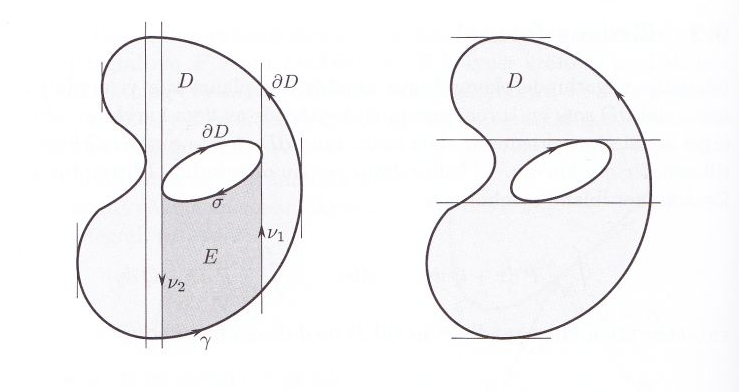
\includegraphics[scale=0.5]{linus_0001.jpg}
	{\it Figur 1}
\end{center}
Inledningsvis visas det att:
$$\int_{\partial E} P \; dx = \iint_E - \frac {dP} {dy} \; dx \; dy$$
$$\iint_E - \frac {dP} {dy} \; dx \; dy = \int^b_{x=a} \left [ -P (x, y) \right ]^{x = \varphi(x)}_{x= \psi(x)} \; dx$$
\begin{align}
	\int_a^bP(x, \psi(x)) \; dx - \int_b^aP(x, \varphi(x)) \; dx
\end{align}
Kurvan $\gamma$ i figuren kan framställas med $x$ som parameter:
$$\gamma = (x, \psi(x)), a\le x \le b.$$
Den första integralen i $(1)$ kan därför skrivas som 
$$\int_{\gamma} P \; dx + 0 \; dy = \int_{\gamma} P \; dx. \; (2)$$
På samma sätt får vi för den andra termen att:
$$- \int_a^b P(x, \varphi(x)) \; dx = \int_{\sigma} P \; dx \; (3)$$ %vad är det här för en variabel?
då kurvintegralen av de (eventuella) randstyckena $v_1$ och $v_2$ är noll innebär detta att
addition av $(2)$ och $(3)$ ger $\int_{\partial E} P \; dx$, vilket
innebär att:
$$\int_{\partial E} P \; dx = \iint_E - \frac {dP} {dy} \; dx dy.$$
genom att addera ihop det här resultatet för alla uppkommande områden av $E$ ger detta:
$$\int_{\partial D} P \; dx = \iint_D - \frac {dP} {dy} \; dx dy.$$
Om vi gör på samma sätt med en uppdelning av $D$ med linjer parallella med X-axeln får vi på liknande sätt att:
$$\int_{\partial D} Q \; dy = \iint_D \frac {dQ} {dx} \; dy dx.$$ 
genom att addera uttrycken följer nu att:
$$\iint_D \left ( \frac {dQ} {dx} - \frac {dP} {dy} \right ) \; dx dy = \int_{\partial D} P \; dx + Q \; dy.$$
\hfill \qed
\paragraph{Definition 2:} En funktion $f$ är analytisk i ett område $D$ om den har en derivata i alla punkter i $D$.\\
\\
\paragraph{Sats 4:} Om $\Gamma$ är en sluten kurva i det komplexa talplanet och $f(z)$ är analytisk i området som innesluts av $\Gamma$ så är:
$$\int_{\Gamma} f(z) \; dz = 0.$$
\\
{\bf Bevis:}\\
Med den vanliga notationen:\\
$f(z) = u(x, y) + iv(x, y)$ får vi:
$$\int_{\Gamma} f(z) \; dz = \int_a^b f(z(t)) \frac {dz(t)} {dt} \; dt = \int_a^b [a(x(t), y(t)) + iv(x(t), y(t)) ]
\left ( \frac {dx} {dt} + i \frac {dy} {dt} \right ) \; dt$$

$$= \int_a^b \left [a(x(t), y(t)) \frac {dx} {dt} - v(x(t), y(t)) \frac {dy} {dt} \right ] \; dt + i \int_a^b \left [v(x(t), y(t)) \frac {dx} {dt} + 
u(x(t), y (t)) \frac {dy} {dt} \right ] \; dt$$

$$\int_{\Gamma} f(z) \; dz = \int_\Gamma (u \; dx - v \; dy) + i \int_\Gamma v \; dx + u \; dy$$
Sats 3 ger nu:
$$\int_{\Gamma} f(z) \; dz = \iint_{D^\prime} \left ( - \frac {dv} {dx} - \frac {du} {dy} \right ) \; dxdy +
i \iint_{D^\prime} \left ( \frac {du} {dx} - \frac {dv} {dy} \right ) \; dxdy$$

där $D'$ är området som innesluts av $\Gamma$. Men ekvationerna från Sats 2 ger nu att
dubbelintegralerna är $0$. vilket ger:
$$\int_\Gamma f(z) \; dz = 0$$
\hfill \qed

\paragraph{Sats 5:} $f(z_0) = \frac 1 {2\pi i} \cdot \int_\Gamma \frac {f(z)} {z - z_0} \; dz$ \\
\\
{\bf Bevis:}\\
$\frac {f(z)} {z - z_0}$ är analytisk överallt i området som innesluts av $\Gamma$ förutom i punkten
$z = z_0$. Vi kan därför deformera $\Gamma$ till en cirkel $C_r$ med radien $r$ och 
som är centrerad kring $z_0$.

\[ \int_\Gamma \frac {f(z)} {z - z_0} \; dz = \int_{C_r} \frac {f(z)} {z - z_0} \; dz. \]

\[ \int_{C_r} \frac {f(z)} {z - z_0} \; dz = \int_{C_r} \frac {f(z) - f(z_0) + f(z_0)} {z - z_0} \; dz =
	\int_{C_r} \frac {f(z_0)} {z - z_0} \; dz + \int_{C_r} \frac {f(z) - f(z_0)} {z - z_0} \; dz \;(1) \]

substitutionen 
\begin{align*}
	z  &= r \cdot e^{iv} + z_0 \\
	dz &= r \cdot i \cdot e^{iv} \; dv
\end{align*}
ger i den vänstra integralen:
\[ \int_{C_r} \frac {f(z_0)} {z - z_0} \; dz = \int_0^{2\pi} \frac {f(z_0) \cdot r \cdot i \cdot e^{iv} } { r \cdot e^{iv}} \; dv =
	\left [f(z_0) \cdot iv \right ]_0^{2\pi} = f(z_0) \cdot 2 \pi i. \]

den högra integralen i $(1) \rightarrow 0$ då radien av cirkeln $\rightarrow 0$.
Detta visas genom att sätta $M_r := \operatorname{max} [|f(z) - f(z_0)|; z \text{ på } C_r]$
Detta innebär att

\[
	\left | \frac {f(z) - f(z_0)} {z - z_0} \right | = \frac {|f(z) - f(z_0)|} {r} \leq \frac {M_r} {r}
\]

\[
	\left | \int_{C_r} \frac {f(z) - f(z_0)} {z - z_0} \; dz \right | \leq \frac {M_r} {r} l(C_r)
\]
där $l(C_r)$ är längden av kurvan $C_r$.

\[
\frac {M_r} {r} \cdot l(C_r) = \frac {M_r} {r} \cdot 2r\pi = M_r \cdot 2 \pi
\]
men då $f$ är kontinuerlig i punkten $z_0$ går $M_r \rightarrow 0$ då $r \rightarrow 0$.
Alltså är $\int_{C_r} \frac {f(z) - f(z_0)} {z - z_0} \; dz = 0.$ Vilket innebär att $(1) = 2\pi i \cdot f(z_0) + 0$
division med $2\pi i$ ger:
\[
	f(z_0) = \frac {1} {2 \pi i} \cdot \int_{\Gamma} \frac {f(z)} {z - z_0} \; dz.
\]
\hfill \qed
\\

\paragraph{Sats 6:}
\[
	f^{(n)}(z_0) = \frac {1} {2 \pi i} \cdot \int_{\Gamma} \frac {f(z)} {(z - z_0)^{(n + 1)}} \; dz \cdot n!
\]
\\
{\bf Bevis:}\\
Detta inses genom att derivera uttrycket med avseende på $z_0$.
\begin{align*}
	f(z_0) &= \frac {1} {2 \pi i} \cdot \int_{\Gamma} \frac {f(z)} {(z - z_0)} \; dz = \frac {1} {2 \pi i} \cdot \int_{\Gamma}
		f(z) \cdot (z - z_0)^{-1} \; dz \\
	f'(z_0) &= \frac {1} {2 \pi i} \cdot -1 \cdot -1 \cdot \int_{\Gamma} f(z) \cdot (z - z_0)^{-2} \; dz \\
	f''(z_0) &= \frac {1} {2 \pi i} \cdot -1 \cdot -2 \cdot \int_{\Gamma} f(z) \cdot (z - z_0)^{-3} \; dz \\
	f'''(z_0) &= \frac {1} {2 \pi i} \cdot 2 \cdot -1 \cdot -3 \cdot \int_{\Gamma} f(z) \cdot (z - z_0)^{-4} \; dz \\
	\vdots \\
	f^{(n)}(z_0) &= \frac {1} {2 \pi i} \cdot n! \cdot \int_\Gamma f(z) \cdot (z \ z_0)^{-(n + 1)} \; dz
\end{align*} %jag fattade inget av Sats 5, jag tror att det är fel
\hfill \qed
\\
\paragraph{Sats 7:}
\[
	f(z) = \sum_{j = - \infty}^\infty a_j (z - z_0)^j. \text{ med } a_j = \frac {1} {2 \pi i} \cdot \ointctrclockwise
		\frac {f(\zeta)} {(\zeta - z_0)^{j + 1}} \; d\zeta
\]
Detta kallas för en Laurent-serie\\
\\
{\bf Bevis:}\\
Låt $\Gamma$ vara en sluten kurva runt $z$.
Låt därefter $\Gamma$ se ut som en ``donut'' med en ``bit'' borta.
%biiild
\begin{center}
	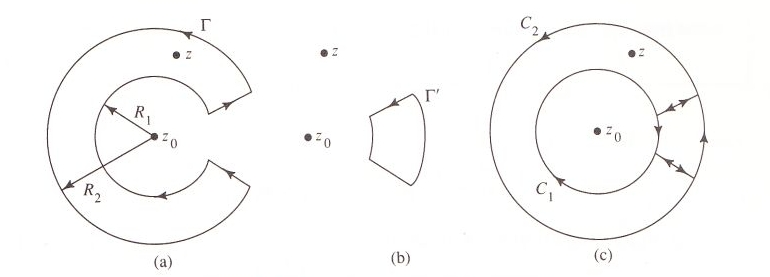
\includegraphics[scale=0.5]{aoeu.jpg}
	{\it Figur 2}
\end{center}
Låt $\Gamma'$ vara den ``borttagna biten''. då $f(z)$ är analytisk i hela området som innesluts av $\Gamma'$ ger Sats 3 att.
\[
	\frac {1} {2 \pi i} \int_{\Gamma'} \frac {f(\zeta)} {\zeta - z} \; d\zeta = 0
\]
därmed följer att vi kan ``sätta tillbaka biten''. Då integralen var $= 0$ följer att:
\[
	f(z) = \frac {1} {2 \pi i} \cdot \int_{\Gamma + \Gamma'} \frac {f(\zeta)} {\zeta - z} \; dz
\]
då integralerna längs linjesegmenten tar ut varandra följer det att:
\[
	f(z) = \frac {1} {2 \pi i} \left ( \varointclockwise_{C_1} \frac {f(\zeta)} {\zeta - z} \; d\zeta + 
		\ointctrclockwise_{C_2} \frac {f(\zeta)} {\zeta - z} \; d\zeta \right ) \quad (1)
\]
\[
	f(z) = \sum_{k = 0}^\infty \frac {f^{(n)}(z_0)} {n!} (z - z_0)^n \quad \text{ (taylorpolynom) }
\]

Sats 6 ger nu:
\[
	f(z) = \sum_{n = 0}^\infty a_n (z - z_0)^n = \frac {1} {2 \pi i} \cdot \ointctrclockwise_{C_2} \frac 
		{f(\zeta)} {\zeta - z} \; d\zeta
\]
Om man nu fokuserar på integralen runt $C_1$ i $(1)$ så ser man att då $z$ ligger utanför $C_1$ 
måste vi integrera kring en annan punkt.
\[
	\frac {1} {\zeta - z} = \frac {1} {(\zeta - z) - (z - z_0)} = - \frac {1} {(z - z_0)}
		\left (
			\frac {1} {1 - \frac {(\zeta - z_0)} {(z - z_0)}}
		\right )
\]
taylorpolynomet till den högra faktorn ger nu:
\[
	- \frac {1} {(z - z_0)} \cdot \sum_{k = 0}^\infty
		\left (
			\frac {(\zeta - z_0)} {(z - z_0)}
		\right )^k
\]
insättning i integralen ger nu:
\[ %wuuuut
	- \frac {1} {2 \pi i} \varointclockwise_{C_1} f(\zeta) \cdot \sum_{k = 1}^\infty \frac {(\zeta - z_0)^{k - 1}} {(z - z_0)^k} \; d\zeta
	= \sum_{k = 1}^\infty -\frac{1} {2 \pi i} \cdot \varointclockwise_{C_1} \frac {f(\zeta)} {(\zeta - z_0)^{-k + 1}} \; d\zeta \cdot
			(z - z_0)^{-k} = \sum_{k = 1}^\infty a_{-k} (z - z_0)^{-k}
\] %överväg radbrytning
Där $a_{-k} = -\frac{1} {2 \pi i} \cdot \varointclockwise_{C_1} \frac {f(\zeta)} {(\zeta - z_0)^{-k + 1}} \; d\zeta$.
%\[
%	= \sum_{k = 1}^\infty a_{-k} (z - z_0)^{-k}
%\]
Ekvation $(1)$ blir nu:
\[
	\sum_{n = 0}^\infty a_n(z - z_0)^n + \sum_{k = 1}^\infty a_{-k}(z - z_0)^{-k}
\]
\hfill \qed

\paragraph{Sats 8:}
Om $f$ har en singularitet i punkten $z_0$ så är linjeintegralen runt singulariteten $= 2 \pi i \cdot a_{-1}$.\\
\\
{\bf Bevis:}\\
Sats 7 ger att $f(z) = \sum\limits_{j = - \infty}^\infty a_j (z - z_0)^j$
\[
	\ointctrclockwise_{C_r} f(z) \; dz = \sum_{j = - \infty}^\infty a_j \cdot \ointctrclockwise_{C_r} (z - z_0)^j \; dz
\]
\begin{align*}
	z &= e^{iv} + z_0 \\
	dz &= ie^{iv} dv \qquad \text{ för } j \neq - 1
\end{align*}
\[
	\ointctrclockwise_{C_r} (z - z_0)^j \; dz = \int_0^{2 \pi} ie^{ir(j + 1)} \; dv =
	\left [
		i \frac {e^{iv(i + 1)}} {i (j + 1)}
	\right ]_0^{2 \pi}
	= 0
\]
\[
	\text{för } j = -1 \text{ gäller: } \int_0^{2\pi} ie^{iv(-1 + 1)} \; dv = 
	\left [
		i \cdot v
	\right ]_0^{2\pi}
	= 2 \pi i
\]
för alla $j \neq -1$ blir integralen $ = 0$ och för $j = -1$ blir integralen lika med $2 \pi i a_{- 1}$.
Alltså:
\[
	\ointctrclockwise_{C_r} f(z) \; dz = 2 \pi i \cdot a_{-1}
\]
där termen $a_{-1}$ kallas för residualen \\
\hfill \qed

\paragraph{Sats 9:} $a_{-1} = \lim_{z \to z_0} f(z) \cdot (z - z_0)$\\
\\
{\bf Bevis:}\\
Om $f(z)$ har en ``borttagbar'' singularitet i Punkten $z = z_0 \qquad \left ( \frac {1} {z - z_0} \right )$ blir 
alla koefficienter till $f(z)$'s Laurentserie för $j < -1 = 0$. Detta på grund av att integralen i $a_k$ för $k < -1$
inte innesluter en singularitet, och integralen  är därmed, enligt Sats 3, lika med $0$.
Men om $f(z)$ har en singularitet i punkten $z = z_0$ gäller:
\begin{align*}
	&f(z) = \frac {a - 1} {z - z_0} + a_0 + a_1(z - z_0) + a_2(z - z_0)^2 \ldots \\
	&f(z) (z - z_0) = a_{-1} + (z - z_0)(a_0 + a_1 (z - z_0) \ldots ) \\
	\lim_{z \to z_0} &f(z)(z - z_0) = a_{- 1} + (0)(a_0 + a_1(z - z_0) \ldots ) = a_{-1}
\end{align*}
\hfill \qed
\\
\paragraph{Sats 10:} %kanske ska ändra till "implicerar"
Om $A_n = \sum\limits_{i = 0}^n a_1, \quad \text{ då är } \sum\limits_{i = 0}^n a_i \cdot b_i = 
		\sum\limits_{i = 0}^{n - 1} A_i (b_i - b_{i + 1}) + A_n \cdot b_n$\\
{\bf Bevis:}\\
\\
\[ a_k = A_k - A_{k - 1} \]
\[
	\sum_{k = 0}^n a_k \cdot b_k =  \sum_{k = 0}^n (A_k - A_{k - 1}) \cdot b_k = \sum_{i = 0}^n A_k \cdot b_k - 
		\sum_{k = 0}^n A_{k - 1} \cdot b_k
\]
i den andra summan substitueras $k$ mot $i + 1$
\[
	\sum_{k = 0}^n A_{k - 1} \cdot b_k = \sum_{i = 0}^{n - 1} A_i \cdot b_{i + 1} = \sum_{k = 0}^{n - 1} A_k \cdot b_{k + 1}
\]
vi har nu
\[
	\sum_{k = 0}^n a_k \cdot b_k = \sum_{k = 0}^n A_k \cdot b_k - \sum_{k = 0}^{n - 1} A_k \cdot b_{k + 1} =
		\sum_{k = 0}^{n - 1} A_k (b_k - b_{k + 1}) + A_n \cdot b_n
\]
\\
\paragraph{Sats 11:} $(n^{-s} - (n + 1)^{-s}) = s \cdot \int\limits_n^{n + 1} x^{-s - 1} \; dx$\\
{\bf Bevis:}\\
\[
	s \cdot \int_n^{n + 1} x^{-s - 1} \; dx = - [ x^{-s} ]_n^{n + 1} = - ((n + 1)^{-s} - n^{-s})
		= n^{-s} -(n + 1)^{-s}
\]
\hfill \qed
\\
\paragraph{Definition 3:} $\floor{x} = \text{ heltalsdelen av } x$\\
\\
exempel:\\
$\floor{\pi} = 3, \quad \floor{e} = 2, \quad \floor{38.5} = 38$\\
\\
\paragraph{Definition 4:} $\fpart{x} = x - \floor{x}$\\
\\
exempel:\\
$\fpart{\pi} = 0.14159265358979 \ldots, \quad \fpart{e} = 0.72182818284590 \ldots, \fpart{38.5} = 0.5$\\
\\
\paragraph{Sats 12:} $\frac {s} {s - 1} - s \cdot \int\limits_1^\infty \floor{x} x^{-s - 1} \; dx +
		s \cdot \int\limits_1^\infty \fpart{x} x^{-s - 1} \; dx$ \\
{\bf Bevis:}\\
\[
	s \cdot \int_1^\infty x^{-s - 1} (\floor{x} + \fpart{x}) \; dx = s \cdot \int_1^\infty x^{-s} \; dx
\]
\[
	= s \cdot \left [
		\frac {x^{-s + 1}} {-s + 1}
	\right ]_1^\infty =
	\frac {1^{1 - s}} {1 - s} \cdot s = \frac {s} {1 - s}
\]
\hfill \qed
\\
\paragraph{Sats 13:} $\zeta(s) = \frac {s} {s - 1} - s \int\limits_1^\infty \fpart{x} x^{-s - 1} \; dx$\\
\\
{\bf Bevis:}\\
\[
	\zeta(s) = \sum_{n \leq n} \frac {1} {n^{-s}}
\]
Sats 10 ger:
\[
	\sum_{n \leq 1} \frac {1} {n^{-s}} = \sum_{n \leq 1} n \cdot (n^{-s} - (n + 1)^{-s})
\]
Sats 11 ger nu att:
\[
	s \sum_{n \leq 1} n (n^{-s} - (n + 1)^{-s}) = s \sum_{n \leq 1} \int_n^{n + 1} \floor{x} x^{-s -1} \; dx =
		s \int_1^\infty \floor{x} x^{-s - 1} \; dx
\]
Sats 12 ger slutligen att:
\[
	\int_1^\infty \floor{x} x^{-s - 1} \; dx = \frac {s} {s - 1} - s \int_1^\infty \fpart{x} x^{-s - 1} \; dx = \zeta(s)
\]
\hfill \qed
\\
\paragraph{Sats 14:} $\zeta(s)$ har en singularitet i $s = 1$ med residualen $1$.\\
\\
{\bf Bevis:}\\
Sats 9 visar att residualen $= \lim_{z - z_0} f(z)(z - z_0)$
\[
	\zeta(s) - (s - 1) = \left (
		\frac {s} {s - 1} - s \cdot \int_1^\infty \fpart{x} x^{-s - 1} \; dx 
		\right )
	(s - 1)
\]
\[
	\lim_{s \to 1} \zeta(s)(s - 1) = \lim_{s \to 1} s - s (s - 1) \cdot \int_1^\infty \fpart{x} x^{-s - 1} \; dx =
		1 - 0 = 1
\]
\hfill \qed
\pagebreak
\section*{Referenser}
Arne Persson \& Lars-Christer Böiers, (2005), Analys i Flera Variabler. Lunds Studentlitteratur AB.\\
\\
E. B Saff \& A. D. Snider, (1993), Fundamentals of Complex Analysis for Mathematics, Science, And Engineering,
Upper Saddle River, New Jersey:\\
Simon \& Schutser Company.\\
\\
ELias M. Stein \& Rami Shakarchi, (2003), Fourier Analysis An Introduction, Princeton, New Jersey:\\
Princeton University Press.\\
\\
Eric Naslund, (2011), Zeros on the Critical Line [Digital].\\
Tillgänglig:\\
\url{http://www.math.ubc.ca/~gerg/teaching/613-Winter2011/ZerosCriticalLine.pdf}\\
\\
Okänd, (2007), Notes on the Riemann Zeta Function [Digital]\\
Tillgänglig:\\
\url{http://people.math.gatech.edu/~ecroot/riemann\_notes.pdf}\\
\\
Robert B. Nash, (Okänd), Complex Variables (Chapter 7, The Prime Number Theorem) [Digital].\\
Tillgänglig:\\
\url{http://www.math.uiuc.edu/~r-ash/CV/CV7.pdf}
\end{document}



